\section{Boss stage 1: Simple excercise using jQuery}

\begin{frame}[fragile]
  \begin{center}
    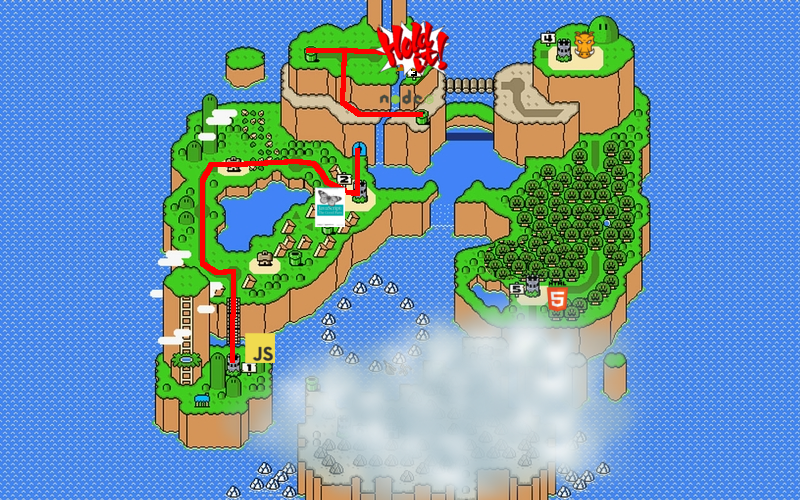
\includegraphics[width=300px]{images/map_boss_stage_1.png}
  \end{center}
\end{frame}

\begin{frame}[fragile]
  \frametitle{Simple exercise using jQuery}
  \begin{block}{Exercise}
    \begin{itemize}
      \item Start with the sample code on tag \texttt{boss\_stage\_1}
      \item Remember to install your dependencies using bower
      \item Create a function for creating \texttt{character} objects
      \item Create another function for creating \texttt{player} objects inheriting from \texttt{characters}
      \item Create another function for creating \texttt{enemy} objects inheriting from \texttt{characters}
      \item Use the jQuery sample code and complete 'Attack' and 'Drink potion' actions.
      \item Use \texttt{console.log} to debug your actions
    \end{itemize}
  \end{block}
\end{frame}
